\documentclass[12pt]{article}
\usepackage{amssymb, amsthm, amsmath, amsfonts, fancybox, multicol, graphicx, 
type1cm, color, array, bardtex, verbatim, tikz, pgfplots}

\usetikzlibrary{shapes.geometric, positioning, automata, arrows.meta}

\tikzset{
	simplex/.pic={
		\newcount\mycount
		\tikzset{state/.style={fill=none, draw=violet, text=black, 
		shape=circle}}
		\pgfmathsetmacro\rot{360.0/\N}
		\begin{scope}[rotate=\rot]
			\node[regular polygon, regular polygon sides=\N,
				minimum size=\radius, rotate=\rot] (A) {};
			\pgfmathsetmacro\None{\N-1}
			\foreach \i in {1,...,\N}
			\node[state] (\i) at (A.corner \i) {\i};
			
			\foreach \i in {1,...,\None}{
				\mycount=\i
				\advance\mycount by 1
				\foreach \j in {\the\mycount,...,\N} {
					\draw[-{Stealth[scale=1.5,angle'=45]},semithick] (\i) -- (\j);
				}
			}
		\end{scope}
	},
	N/.store in=\N,
	radius/.store in=\radius,
	radius=10cm,
	N=5,
}

\graphicspath{{resources/}}

\styleoption{poster}
\posterstyle{stylefour}
\toptitlecolor{Orchid}
\boxcolor{Thistle}
\boxtitlecolor{Periwinkle}

\begin{document}

\begin{posterbard}

	\postertopscale{Neural Network Reconstruction via Graph Locality-Driven 
		Machine Learning}{Hayden Sartoris}{Computer Science}{May 2018}{Sven 
	Anderson, Arseny Khakhalin}{1}

	\begin{posterboxabstract}
		\noindent A ubiquitous problem within the field of computational 
neuroscience is the determination of biological neural network structure and 
connectivity from imaging of stochastic, large-scale network activity. We 
propose an algorithm inspired by convolutional approaches to image processing, 
adapted to the graph structure of neural networks. To achieve this, we redefine 
locality in terms of graph adjacency, and create a scale-independent algorithm 
facilitated by modern machine learning techniques to incorporate this locality 
data into individual connection prediction.
	\end{posterboxabstract}

	\begin{posterboxtitle}{Steps Toward Our Goal}
		\noindent Our goal was to infer biological neural network connectivity 
		from spiking data, itself inferred from calcium imaging of biological 
		networks. To do so, we took the following steps:
		\begin{enumerate}
			\item Considered biological networks in terms of a graph 
				representation
			\item Identified features within that graph representation 
				potentially useful to reconstruction
			\item Created a model based around an algorithm informed by these 
				features and inspired by convolutional neural networks
			\item Generated data from a variety of simple test networks
			\item Trained models on that data and analyzed the resulting output 
				to determine efficacy
		\end{enumerate}
	\end{posterboxtitle}

	\begin{posterbox}
		\begin{center}\textbf{Spike-time Raster Plots}\end{center}
		\begin{itemize}
			\item Matrices of binary data
			\item Each row represents a step in time
			\item Each column represents a neuron over time
		\end{itemize}
		For a three neuron network sampled for eight timesteps, a raster plot 
		might appear as below.
		\begin{center}
			\scalebox{.5}{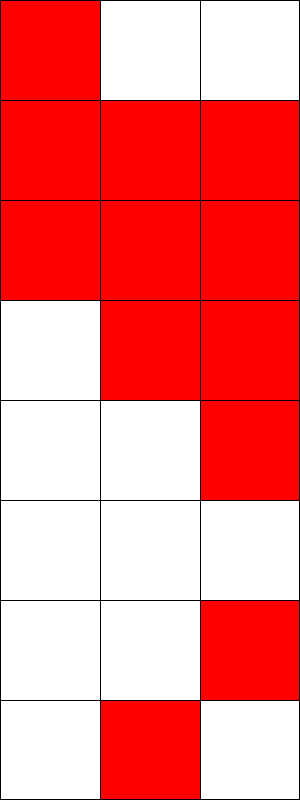
\includegraphics{fullRun/0_py/input.png}}
		\end{center}
		\vspace{\baselineskip}
	\end{posterbox}

	
	\begin{posterboxtitle}{Biological Networks \& Graphs}
		\noindent \textbf{Graph Representation of Neural Networks}
		\begin{itemize}
			\item Biological networks broadly equivalent to directed graphs 
				(diGraphs)
			\item diGraphs consist of nodes and edges, as below
			\item In neural networks, neurons are nodes and connections are 
				edges
			\item Probability of connection between two neurons unrelated to 
				physical proximity
		\end{itemize}\footnote{Cite 11, 3, 13}
		\begin{center}
			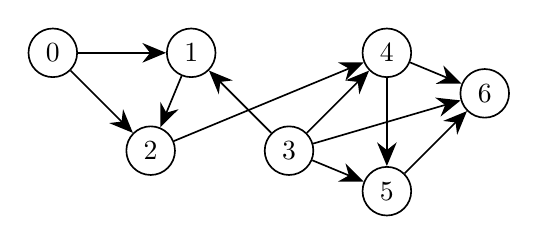
\begin{tikzpicture}[node distance=5em,->,
				-{Stealth[scale=1.5,angle'=45]},semithick]
				\tikzset{state/.style={fill=none, draw=black, text=black,
					shape=circle}}
				\node[state] (0) {0};
				\node[state] (1) [right of=0] {1};
				\node[state] (2) [below right of=0] {2};

				\path 	(0) edge node {} (1)
						(0) edge node {} (2)
						(1) edge node {} (2);
				
				\node[state] (3) [right of=2] {3};
				\node[state] (4) [above right of=3] {4};
				\node[state] (5) [below of=4] {5};
				\node[state] (6) [above right of=5] {6};

				\path 	(3) edge node {} (4)
						(3) edge node {} (5)
						(3) edge node {} (6)
						(4) edge node {} (5)
						(4) edge node {} (6)
						(5) edge node {} (6);

				\path 	(3) edge node {} (1)
						(2) edge node {} (4);
			\end{tikzpicture}
		\end{center}
		\textbf{Common Local Structures}
		\begin{itemize}
			\item Motifs, repeating local structures, unusually common in 
				biological networks
			\item Some motifs, simplices, are structures in which information 
				flows in one direction, from a `source' node to a `sink' node
		\end{itemize}\footnote{Cite 5,9,11}
		An example of a 6-simplex is below; the graph above contains a 2-simplex 
		and a 3-simplex.\\
		\begin{center}
			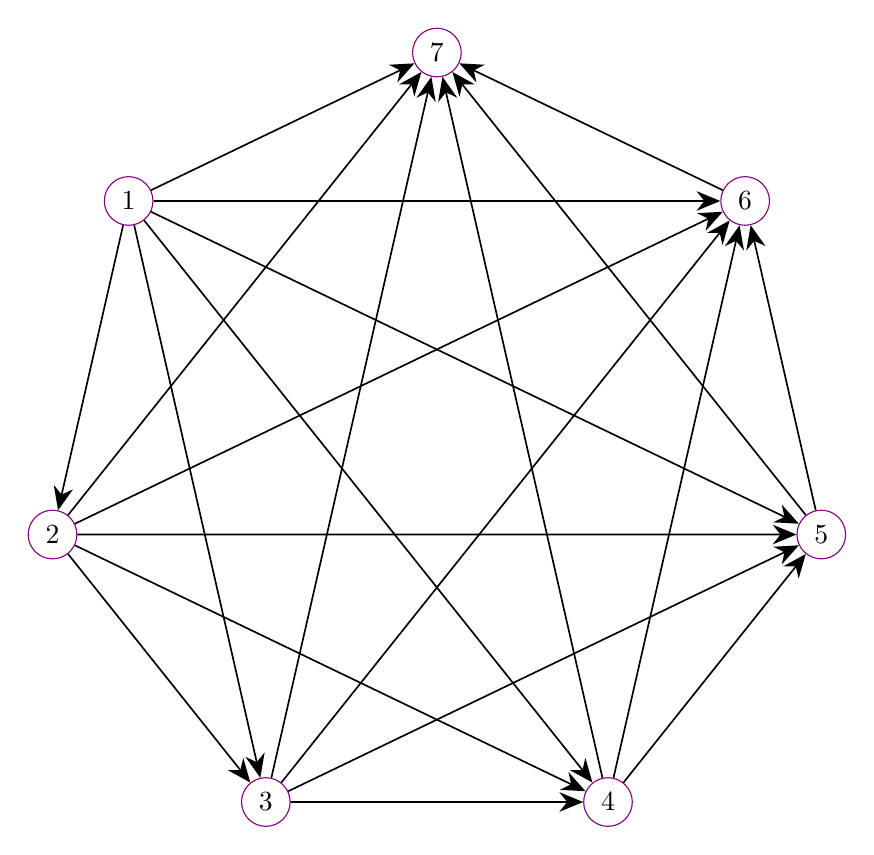
\begin{tikzpicture}
				\pgfmathsetmacro\N{7}
				\pic {simplex={N=\N}};
			\end{tikzpicture}
		\end{center}
	\end{posterboxtitle}
	\begin{posterbox}
		\begin{center}\textbf{Graph Convolution}\end{center}
		\begin{itemize}
			\item Convolutional neural networks are used on data containing many 
				local features, such as images
			\item They involve tranposing a small `filter' matrix across input 
				data, limiting the size of an analysis model to the total size 
				of its filters, instead of the size of input images
			\item In an image, nearby pixels are adjacent; in a graph, connected 
				nodes are adjacent
			\item We designed an algorithm to incorporate information from 
				adjacent nodes in the determination of whether or not a given 
				connection in a network exists
		\end{itemize}
		\vspace{\baselineskip}
	\end{posterbox}
	\begin{posterboxtitle}{Model}
		\noindent\textbf{First Layer}
		\begin{itemize}
			\item Accepts spike-time raster plots for each of \textit{n} neurons
			\item Converts to $(d \times n^2)$ matrix, with each 
				\textit{d}-vector representing one potential edge
			\item Figure here
		\end{itemize}
		\noindent\textbf{Locality Layer}
		\begin{itemize}
			\item Accepts data from the first layer
			\item Incoporates data from potentially adjacent edges into the 
				calculation of the existence of a given edge
			\item Figure here
		\end{itemize}
		\noindent\textbf{Final Layer}
		\begin{itemize}
			\item Converts output from locality layer into $(n \times n)$ 
				adjacency matrix
			\item figure also here
		\end{itemize}
	\end{posterboxtitle}


\end{posterbard}

\end{document}
